\documentclass{report}

% ----------------------------------------------------
% PACKAGE
% ----------------------------------------------------

\usepackage{graphicx}
\usepackage{amsmath}
\usepackage{amsfonts}
\usepackage{amssymb}
\usepackage{tocloft}
\usepackage{amsthm}
\usepackage{hyperref}
\usepackage[a4paper, portrait, margin=0.75in]{geometry}
\usepackage[italian]{babel}
\usepackage{enumerate}% http://ctan.org/pkg/enumerate


\hypersetup{
    colorlinks=true,
    linkcolor=black,
    urlcolor=blue,
}

\title{Fondamenti di controlli automatici \\[1ex] \large Un goliardico riassunto}
\author{Ollari Dmitri}

\begin{document}
\newtheorem*{theorem}{Teorema}
    \maketitle
    
    \tableofcontents

    \chapter{Il controllo attivo di un processo}

Un processo \`e l'evoluzione nel tempo di un sistema.

Con controllo attivo si intende una strategia di controllo del sistema controllato che prevede 
un'azione di controllo che dipende dallo stato del sistema stesso.

\section{Insieme dei Behaviors}

I behaviors sono tutte le possibile coppie causa-effetto associate ad un'sistema.








    \chapter{Modellistica ed equazioni differenziali lineari}

\section{Circuiti elettrici}

\begin{center}
  \begin{tabular}{|l l|}
  \hline
    Resistenza & $v(t) = Ri(t)$ \\
    Induttanza & $v(t) = L\frac{di(t)}{dt} = LDi$ \\
    Capacità & $v(t) = \frac{1}{C}\int_{-\infty}^t i(\tau) \rightarrow Dv_C = \frac{i}{C}$ \\
  \hline
  \end{tabular}
\end{center}

\section{Sistema meccanico}
\begin{center}
  \begin{tabular}{|l l|}
  \hline
    Massa & $MD^2x(t) = f_1(t)-f_2(t)$ \\
    Molla & $f(t) = K(x_1(t) - x_2(t))$ \\
    Ammortizzatore & $f(t) = BD(x_1(t) - x_2(t))$ \\
    \hline
  \end{tabular}
\end{center}



\section{OPAMP}
\begin{figure}[h!]
\centering
  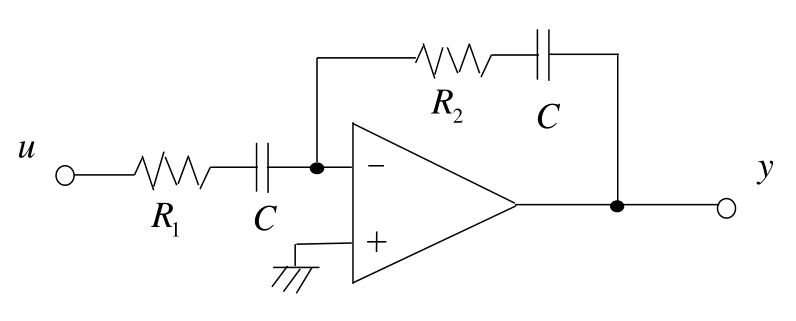
\includegraphics[width=0.4\linewidth]{images/opamp.png}
\end{figure}
Avendo $u$ tensione in ingresso e $y$ tensione in uscita, si ha che:
\begin{align}
  R_1CD_y + y = -R_2CDu - u
\end{align}


\section{Equazioni differenziali lineari}
Generalmente si ha che:

\begin{align}
  \sum_{i=0}^n a_iD^iy = \sum_{i=0}^m b_iD^iu
\end{align}

Dove:
\begin{itemize}
  \item $\rho = |n - m|$ ordine relativo o grado relativo
  \item $y$ è l'uscita
  \item $u$ è l'ingresso
\end{itemize}

\end{document}

